\documentclass{BeamerTemplate}

\title{Module 11 - Régression linéaire multiple}

\graphicspath{{Images/Module 11/}}

\begin{document}
\begin{frame}[t]
  \titlepage
\end{frame}

%-------------------------------------------------------------------------------------------------------------------------------------





%%%%%%%%%%%%%%%%%%%%%%%%%%%%%%%%%%%
%%%%%%%%%%%%%%%%%%%%%%%%%%%%%%%%%%%
%%%%%%%%%%%%%%%%%%%%%%%%%%%%%%%%%%%

\section[Intro]{Introduction}
\subsection*{}

\begin{frame}[t]{Contexte}

\begin{enumerate}\itemsep4mm
\item Plusieurs variables explicatives disponibles.
\item A-t-on au moins une variable significative?
\item Quelle proportion de la variabilité de $Y$ est expliquée par toutes ces variables globalement?
\item Devrait-on utiliser toutes les variables disponibles pour prédire $Y$ avec plus de précision?
\item Lesquelles ont un impact significatif sur $Y$?
\end{enumerate}
% {\small Dans bien des situations, l'analyste aura à sa disposition \alert{plus qu'une variable explicative} $\Rightarrow$ Il serait intéressant de pouvoir utiliser la valeur de \alert{toutes les variables afin de prédire/expliquer la valeur observée de la variable réponse}.

% Nous avons donné un exemple où la variable réponse était la durée de vie des lignes de peinture sur l'asphalte et la variable explicative était la température d'application de la peinture. Peut-\^etre qu'en tenant compte de la valeur d'autres variables, comme le volume de trafic, la concentration d'un additif dans la peinture, il serait possible de prédire de fa\c{c}on plus précise la durée de vie de ces lignes de peinture.}}
\end{frame}


\begin{frame}[t]{Les données}
\begin{itemize}
\item $n$ unités expérimentales indépendantes;
\item  une variable réponse $Y$;
\item  $k$ variables explicatives $X_1,\ldots,X_k$.
\end{itemize}

\bigskip
Les données sont de la forme
$$(Y_1,\;X_{11},\;\ldots,\;X_{1k})$$
$$(Y_2,\;X_{21},\;\ldots,\;X_{2k})$$
$$\ \ ... \ \ \ \ \ \ $$
$$(Y_n,\;X_{n1},\;\ldots,\;X_{nk})$$
\end{frame}
\section[Modèle]{Le modèle}

\subsection{Formulation du modèle}

\begin{frame}[t]{Modèle de régression linéaire multiple}

%{\small
Extension du modèle de régression linéaire simple. \\
\alert{Ici, la  moyenne de $Y$ dépend de plusieurs variables explicatives}.

\begin{Boite}{Modèle de régression linéaire multiple (RLM)}
%Soit $n$ observations indépendantes d'une variable réponse $Y$ et de \\$k$ variables explicatives $X_1,\ldots,X_k$. Le modèle de régression linéaire multiple suppose que
$$
Y_i=\underbrace{\beta_0+\beta_1X_{i1}+\cdots+\beta_kX_{ik}}_{E(Y)=\text{hyperplan}}+E_i,
$$

où $E_1,\ldots,E_n$ sont indépendantes de loi $N(0,\sigma^2)$.
\end{Boite}


Il est possible d'écrire ce modèle de façon matricielle

$$\boldsymbol{Y}=\boldsymbol{X\beta}+\boldsymbol{\epsilon},$$
où $\boldsymbol{Y}$ est le vecteur des $n$ réponses, $\boldsymbol{X}$ est la matrice des variables explicatives, $\boldsymbol{\beta}$ est le vecteur des $k+1$ paramètres et $\boldsymbol{\epsilon}$ est le vecteur des $E_i$
\end{frame}

\begin{comment}


# Régression sans interaction

set.seed(2132)
x1<-seq(0,40,length=30)
x2<-seq(0,40,length=30)

X1<-runif(30,0,40)
X2<-runif(30,0,40)
y<-c(200-4*X1+3*X2+rnorm(30,mean=0,sd=75))
reg<-lm(y~X1+X2)
B<-coefficients(reg)
summary(reg)

mod <- function(x1,x2){
  pred<-B[1]+B[2]*x1+B[3]*x2
  return(pred)
}

z <- outer(x1,x2,mod)

donnees<-data.frame(X1,X2,y,predict.lm(reg))
png("plan.png",width=8,height=6,unit="in",res=90)
par(mar=c(3,1,1,1))
graphe<-persp(x1, x2, z, main = " ",
              theta = 105, phi = 20, r = 10, d = 1, expand = 0.7, col="red",
              ltheta = 90, lphi = 180, shade = 0.1, ticktype = "detailed", nticks=5,
              border=gray(0.4),zlim=c(0,400),
              zlab="y", xlab="x1",ylab="x2",cex.axis=0.8,cex.main=0.8)
noir<-donnees[y>=predict.lm(reg),]# les points au-dessus du plan seront en noir
pts_noir<-trans3d(noir$X1,noir$X2,noir$y,pmat=graphe)
pred_noir<-trans3d(noir$X1,noir$X2,noir$predict.lm.reg,pmat=graphe)

gris<-donnees[y<predict.lm(reg),]# les points sous le plan seront en gris
pts_gris<-trans3d(gris$X1,gris$X2,gris$y,pmat=graphe)
pred_gris<-trans3d(gris$X1,gris$X2,gris$predict.lm.reg,pmat=graphe)
points(pts_noir,pch=19)
segments(x0=pts_noir$x,y0=pts_noir$y,
         x1=pred_noir$x,y1=pred_noir$y)
points(pts_gris,pch=19,col=gray(0.3))
segments(x0=pts_gris$x,y0=pts_gris$y,
         x1=pred_gris$x,y1=pred_gris$y,col=gray(0.3))
dev.off()
\end{comment}
\begin{frame}[t]{Interprétation géométrique}

{\small
Avec $k=2$ variables explicatives $\Rightarrow$ le nuage des points $(x_{i1},x_{i2},y_i)$
sera distribué de façon aléatoire $N(0,\sigma^2)$ autour du plan $y=\beta_0+\beta_1x_1+\beta_2x_2.$
}
\begin{center}
    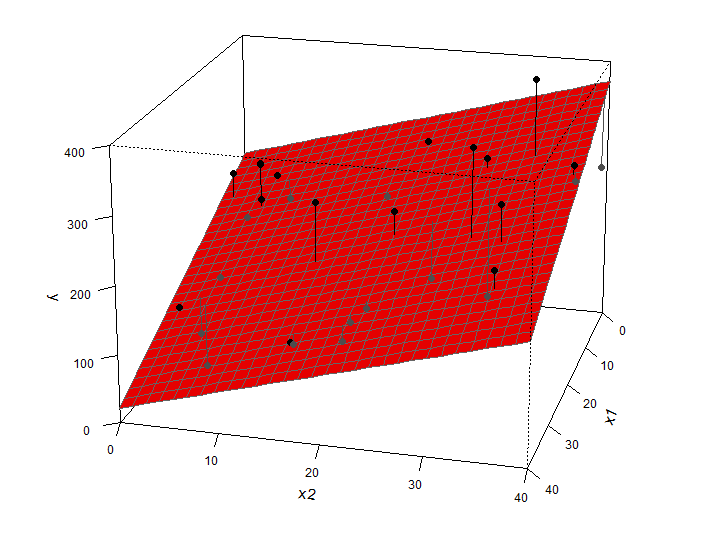
\includegraphics[height=5.2cm]{plan.png}

\end{center}
%\includegraphics[height=4.15cm]{rlm.jpg}

{\small
Si $k>2$, le modèle est un "hyperplan"  $y=\beta_0+\beta_1x_1+...+\beta_kx_k.$
}

\end{frame}


\begin{frame}[t]{Postulats du modèle}

{\small
Les m\^emes 4 postulats qu'avec une variable explicative:
\begin{itemize}\itemsep3mm
\item[P1] {\bf  linéarité:} l'espérance de $Y_i$ est linéaire en $X_{i1},\ldots,X_{ik}$;\\
    {\color{gray}{ $E(Y_i)=\beta_0+\beta_1X_{i1}+\ldots+\beta_kX_{ik} \hspace{0.2cm} \Leftrightarrow  \hspace{0.2cm} E(E_i)=0$ }}
\item[P2] {\bf homoscédasticité:}  la variance de $Y_i$ autour du plan est homogène (elle ne dépend pas des $X_{ij}$);\\
    {\color{gray}{$V(Y_i)=\sigma^2 \hspace{0.2cm} \Leftrightarrow  \hspace{0.2cm} V(E_i)=\sigma^2$}}
\item[P3]  {\bf indépendance:}  les observations sont indépendantes;\\
    {\color{gray}{ $Y_i$ indépendants \hspace{0.2cm} $\Leftrightarrow$  \hspace{0.2cm} $E_i$  indépendants}}
\item[P4]  {\bf  normalité:} les $Y_i$ sont de loi normale autour du plan.\\
    {\color{gray}{  \hspace{0.2cm} $\Leftrightarrow  \hspace{0.2cm} E_i$\  de loi normale autour de 0}}
\end{itemize}
}

{Nous pouvons vérifier ces postulats à l'aide des résidus de manière similaire à
ce qui a été fait à la fin du module précédent.}
\end{frame}

\subsection{Interprétation des paramètres}

\begin{frame}[t]{Interprétation des paramètres}

{\small
Quand toutes les variables entrent linéairement dans le modèle,

$$Y=\beta_0+\beta_1X_1+...+\beta_kX_k+E,$$

les coefficients de régression $\beta_0,\ldots,\beta_k$ s'interprètent comme suit:
\bigskip

%de manière similaire à leur interprétation dans le modèle de régression linéaire simple:
\begin{itemize}\itemsep1cm
\item[$\beta_0$: ] Valeur \alert{moyenne} de $Y$ lorsque $X_1,\ldots,X_k$ prennent \alert{simultanément} la valeur 0.
\item[$\beta_j$: ] Hausse \alert{moyenne} de $Y$ lorsque $X_j$ augmente d'une unité et que les
valeurs des autres variables sont prises en compte mais demeurent \underline{inchangées}.
\end{itemize}
}
\end{frame}



\begin{frame}[t]{Illustration — Génie du bois}

Soit le modèle linéaire :

$$
Y = 35 + 1{,}8\,X_1 - 2{,}4\,X_2 + 0{,}9\,X_3 + E
$$

\vspace{0.4cm}

\begin{tabular}{rl}
$Y$ : & résistance à la flexion (en MPa) \\
$X_1$ : & densité du panneau (kg/m³) \\
$X_2$ : & teneur en humidité (\%) \\
$X_3$ : & proportion de colle structurale utilisée (\%)
\end{tabular}

\vspace{0.4cm}

\begin{itemize}
\item Si la teneur en humidité augmente de 1\%, toutes choses égales par ailleurs, la résistance moyenne **diminue de 2,4 MPa**.
\item Si la densité du panneau augmente de 1 kg/m³, la résistance augmente en moyenne de **1,8 MPa**.
\end{itemize}

\vspace{0.3cm}
{\tiny Ce type de modèle peut être utilisé pour optimiser les conditions de fabrication.}
\end{frame}


\subsection{Estimation des paramètres}

\begin{frame}[t]{Estimation ponctuelle des coefficients $\beta_j$}
Les  $\beta_0,..., \beta_k$ sont estimés en minimisant la somme des carrés des erreurs :

\alert{
$$\begin{array}{ll}
SS_E&=\sum\limits_{i=1}^n(Y_i-\hat Y_i)^2\\
&=\sum\limits_{i=1}^n(Y_i-[\hat{\beta}_0+\hat{\beta}_1X_{i1}+\cdots+\hat{\beta}_kX_{ik}])^2
\end{array}
 $$
 }

En version matricielle, le vecteur des paramètres estimés est
$$\boldsymbol{\hat\beta=(X'X)^{-1}X'Y}$$

On en déduit que les $\hat\beta_j$ sont des combinaisons linéaires des $Y_i$, et donc qu'ils suivent une loi normale.\\

({\it Nous ne faisons pas ces calculs à la main.})
\end{frame}

\begin{frame}[t]{Exemple 1: consommation d'essence per capita}


Weisberg étudie la consommation d'essence des 48 états continentaux
des États-Unis en 1971. Soit
\begin{itemize}
\item[] $Y_i$: la consommation d'essence (gallons par habitant) dans l'état $i$;
\item[] $X_{i1}$: les taxes sur l'essence en vigueur dans l'état $i$ (en cents/gallon);
\item[] $X_{i2}$: le pourcentage de la population de l'état $i$ possédant un permis
de conduire;
\item[] $X_{i3}$: le revenu annuel per capita (en milliers \$) dans l'état $i$;
\item[] $X_{i4}$: la longueur  des routes fédérales (milliers de miles) dans l'état $i$.
\end{itemize}

\end{frame}

\begin{frame}[t]{Exemple 1}

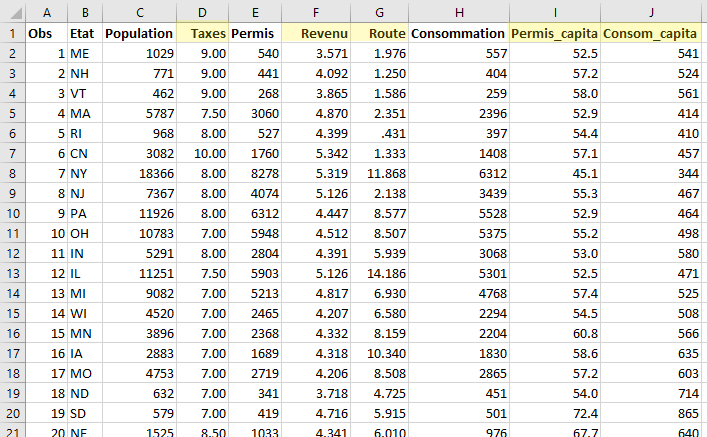
\includegraphics[width=11cm]{essence-data.png}
\end{frame}
\begin{frame}[t]{Exemple 1}

D'après cette matrice de corrélation entre les variables, quelle serait la meilleure variable prise seule pour prédire $Y$?

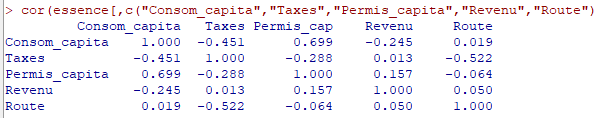
\includegraphics[width=9cm]{essence-cor.png}

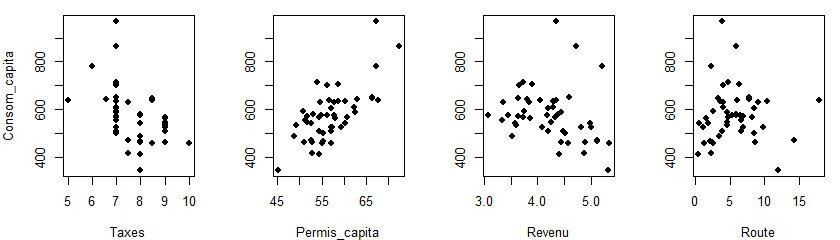
\includegraphics[width=11cm]{yx.png}

\medskip
Peut-on en déduire les 2 meilleures variables? \\ Le meilleur modèle à plusieurs variables?

\end{frame}
\begin{frame}[t]{Exemple 1}

Si on inclut toutes les variables dans le modèle:\\

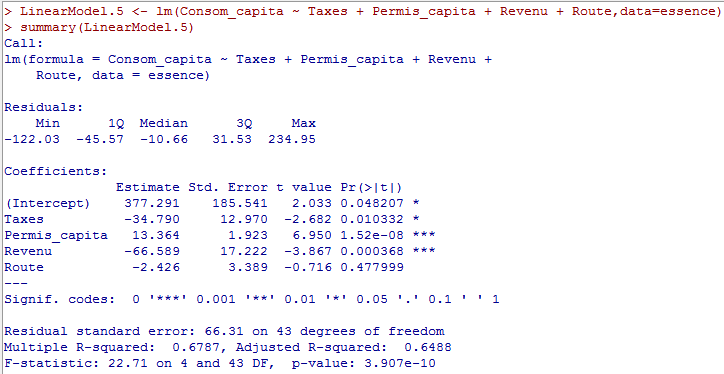
\includegraphics[width=11.5cm]{essence-rlm.png}
\end{frame}

\begin{frame}[t]{Exemple 1: }

L'équation de l'hyperplan estimé est

$$\hat{Y}=377,29-34,79X_{1}+13,36X_{2}-66,59X_{3}-2,43X_{4}.$$

\underline{Interprétation de $\hat\beta_1$ }:

\medskip

Si on augmente la taxe sur l'essence de 1 cent par gallon, mais qu'\alert{on ne change pas la valeur des autres variables}, alors la consommation d'essence annuelle moyenne devrait diminuer de $34,79$ gallons par habitant.

\bigskip


\end{frame}

\begin{frame}[t]{ }

\centerline{\LARGE\bf \alert{REMARQUE}}
\bigskip



\begin{itemize}\itemsep1cm

\item Si on retire une variable du modèle (p.ex. $X_4$) du modèle, les estimations des coefficients de régression pour les autres variables (p.ex. $\beta_1,\,\beta_2,\,\beta_3$) sont susceptibles de changer.

\item Si on garde le même échantillon, l'estimation de l'ordonnée à l'origine $\beta_0$ va changer selon les variables que l'on inclut dans le modèle.

    \vspace{1cm}
    \end{itemize}

\end{frame}


\section{Inférence}

\subsection{Test global du modèle de régression}

\begin{frame}[t]{1) Test simultané de tous les coefficients}
Première question importante en régression linéaire multiple:
\bigskip

\begin{center}
\textit{``Est-ce  qu'au moins une des variables explicatives est associée à la variable réponse?}''
\end{center}

\alert{1) Test global de la régression}.

\begin{align*}
H_0:&~\beta_1=\cdots=\beta_k=0\\
H_1:&~\text{au moins un paramètre parmi\ }\beta_1,\ldots,\beta_k\text{\  ne vaut pas zéro.}
\end{align*}
\end{frame}

\begin{frame}[t]{Analyse de la variance}

{\small
Ce test s'effectue à l'aide d'une table d'analyse de la variance.

\bigskip
$\begin{array}{lll}
\hat{Y}_i&=\hat{\beta}_0+\hat{\beta}_1X_{i1}+\cdots+\hat{\beta}_kX_{ik}&=\text{la $i^e$ valeur ajustée (ou prédite), }\\[2mm]
e_i&=Y_i-\hat{Y}_i&=\text{le $i^e$ résidu.}
\end{array}$
\bigskip

On définit les sommes de carrés
\bigskip

$\left.\begin{array}{ll}
SS_R&=\sum_{i=1}^n(\hat{Y}_i-\overline{Y})^2\\[3mm]
SS_E&=\sum_{i=1}^n(Y_i-\hat{Y}_i)^2=\sum_{i=1}^ne_i^2\\[3mm]
SS_T&=\sum_{i=1}^n(Y_i-\overline{Y})^2\\
\end{array}\right\}$\begin{tabular}{c}
On peut montrer que\\[5mm] $SS_T=SS_R+SS_E$.\end{tabular}
}
\end{frame}
\begin{frame}[t]{Analyse de la variance}

{\small

\underline{Si $H_0$ est vraie}, les $\beta_j$ sont tous nuls, l'hyperplan est horizontal et
\begin{itemize}
\item les prédictions $\hat Y_i$ sont toutes ``proches'' de la moyenne $\overline Y$;
\item $SS_R$ tend à prendre de faibles valeurs;
\item $F_0=\dfrac{SS_R/k}{SS_E/(n-k-1)}=\dfrac{MS_R}{MS_E}$ suit une loi $F_{k,n-k-1}$.
\end{itemize}

\uncover<2>{

\underline{\hspace{10cm}}\\
\underline{Si $H_1$ est vraie}, certains $\beta_j$ sont non nuls, et
\begin{itemize}
\item les prédictions $\hat Y_i$ changent en fonction des valeurs des $X_{ij}$;
\item $SS_R$ tend à prendre de grandes valeurs;
\item $F_0=\dfrac{MS_R}{MS_E}$ sera beaucoup plus grand que 1.
\end{itemize}

\underline{\hspace{10cm}}\\
On rejettera donc $H_0$ au seuil $\alpha$ si $f_0>F_{\alpha;k,n-k-1}$.
}}
\end{frame}

\begin{frame}[t]{Table d'analyse de la variance}

{\small
\begin{tabular}{cccccc}\hline
Source de & Somme de & Deg. de & Carrés  & $F_0$ & Valeur $p$ \\
variabilité & carrés & liberté & moyens & & \\ \hline
\\
Régression & $SS_{R}$ & $k$ & $MS_{R}=\dfrac{SS_R}{k}$ & $f_0=\dfrac{MS_{R}}{MS_E}$ & $P(F_{k,n-k-1}>f_0)$ \\[5mm]
Erreur & $SS_E$ & $n-k-1$ & $MS_E=\dfrac{SS_E}{n-k-1}$ & & \\ 
\\
\hline
\\
Totale & $SS_T$ & $n-1$ & & & \\ 
\\\hline

\end{tabular}
}

\medskip
\uncover<2->{
{\small
\alert{Si le test $F$ rejette $H_0$}, on sait qu'au moins une des variables explicatives est associée à la valeur de $Y$. Laquelle ou lesquelles des $k$ variables le sont?

$\Rightarrow$ sélection de variables (plus loin).
%$\Rightarrow$ tests partiels  sur les coefficients individuels. (Justement pas... )
}
}
\end{frame}

\begin{frame}[t]{Exemple 2 sur la consommation d'essence}

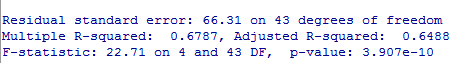
\includegraphics[width=9cm]{essence-rlm-F.png}


{\small
%{\it R Commander} nous donne les valeurs en bleu.


\bigskip
\begin{tabular}{cccccc}\hline
Source de       & Somme de & Degrés de & Carré moyen & $F_0$ & Valeur $P$ \\
variabilité   & carrés  & liberté & & & \\ \hline
Régression    & $399\,425$  & $4$      & $99\,856.32$           & $22.71$ & $3.907\times 10^{-10}$ \\
Erreur          & $189\,072$    & $43$  & $66.31^2 = 4\,397.02$ &                           & \\ \hline
Totale          & $588\,497$    & $47$     &                           &                           & \\ \hline
\end{tabular}


\bigskip
Expliquez pourquoi les données supportent l'hypothèse qu'\textit{au moins une des quatre variables explicatives est associée à la consommation d'essence} (pour tous les seuils usuels).
}
\end{frame}

\subsection{Test partiel sur la valeur d'un coefficient $\beta_j$}

\begin{frame}{Test partiel sur un coefficient $\beta_j$ }

%\textbf{Objectif} : tester si la variable $X_j$ a un effet significatif sur $Y$, \\
\textbf{Objectif} : tester la force de l'effet de la variable $X_j$ sur $Y$, \\
\hspace{1em} \textit{en tenant compte des autres variables du modèle}.

\vspace{0.4cm}

\begin{itemize}
      \item[$H_0$ :] $\beta_j = c$ \hfill \textit{(souvent $c = 0$)} \\
%  \hspace{2em} $\Rightarrow$ Une variation de $X_j$ n’a pas d’effet moyen (supplémentaire) sur $Y$
 \hspace{2em} $\Rightarrow$ Compte tenu de la présence des autres variables, une hausse de 1 unité de $X_j$ fait varier $Y$ de $c$ unités en moyenne 
  \vspace{0.3cm}
  \item[$H_1$ :] $\beta_j \neq c$ \\
%  \hspace{2em} $\Rightarrow$ $X_j$ a un effet sur $Y$, en présence des autres variables
\hspace{2em} $\Rightarrow$ En présence des autres variables, $\beta_j$ diffère de $c$.
\end{itemize}


\end{frame}


\begin{frame}{Statistique de test et IC}

\vspace{-0.2cm}

\textbf{Statistique de test :}

\vspace{0.2cm}

\[
T_0 = \frac{\hat{\beta}_j - c}{\text{se}(\hat{\beta}_j)} \quad \sim t_{n - k - 1} \quad \text{si } H_0 \text{ est vraie}
\]

\vspace{0.3cm}

\textbf{Intervalle de confiance pour $\beta_j$ au niveau $1 - \alpha$ :}

\vspace{0.2cm}

\[
\hat{\beta}_j \ \pm \ t_{\alpha/2; \, n-k-1} \cdot \text{se}(\hat{\beta}_j)
\]

\vspace{0.4cm}

\textbf{Décision :}

\begin{itemize}
  \item On rejette $H_0$ si $|T_0| > t_{\alpha/2; \, n-k-1}$
  \item ou si $c$ ne se trouve pas dans l’intervalle de confiance
\end{itemize}

\end{frame}


\begin{comment}
\begin{frame}[t]{Variance et covariance des estimateurs}

{\small
Certains logiciels rapportent les estimations de la variance des $\hat{\beta}_j$ dans une \alert{matrice de variances-covariances}:
{\footnotesize
$$\widehat{Var}\left(\begin{array}{c} \hat{\beta}_0 \\ \vdots \\ \hat{\beta}_k\end{array}\right)=
\left(\begin{array}{ccccc}
\widehat{Var}(\hat{\beta}_0) & \widehat{Cov}(\hat{\beta}_0,\hat{\beta}_1) & \widehat{Cov}(\hat{\beta}_0,\hat{\beta}_2) & \cdots & \widehat{Cov}(\hat{\beta}_0,\hat{\beta}_k) \\
\widehat{Cov}(\hat{\beta}_1,\hat{\beta}_0) & \widehat{Var}(\hat{\beta}_1)  & \widehat{Cov}(\hat{\beta}_1,\hat{\beta}_2)& \cdots & \widehat{Cov}(\hat{\beta}_1,\hat{\beta}_k) \\
 \vdots &   &   &  & \vdots \\
\widehat{Cov}(\hat{\beta}_k,\hat{\beta}_0) & \widehat{Cov}(\hat{\beta}_k,\hat{\beta}_1) & \widehat{Cov}(\hat{\beta}_{k},\hat{\beta}_2) & \cdots &  \widehat{Var}(\hat{\beta}_k) \\
\end{array}\right).$$
}

L'erreur-type de $\hat{\beta}_j$ est tout simplement $se(\hat{\beta}_j)=\sqrt{\widehat{Var}(\hat{\beta}_j)}$,\\ le terme correspondant sur la diagonale.

\bigskip
Que peut-on déduire des termes hors diagonale de cette matrice?
}
\end{frame}
\end{comment}
\begin{frame}[t]{Exemple 3 sur l'essence}


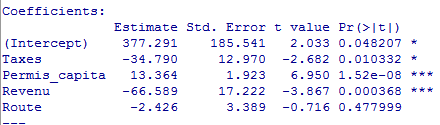
\includegraphics[width=8cm]{essence-rlm-B.png}

\medskip

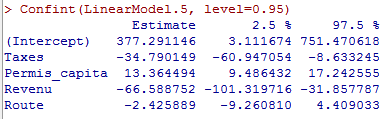
\includegraphics[width=7cm]{essence-coeff.png}

\medskip

\begin{itemize}
\item L'effet d'une hausse de taxes est-il significatif, une fois qu'on tient compte des permis, du revenu et des routes? ($\alpha=0,05$)
\item L'effet d'une hausse de 1\%  des permis diffère-t-il de 10 gallons de plus per capita en moyenne?($\alpha=0,05$)
\end{itemize}
%Le 0 n'appartenant pas à IC($\beta_1$), on sait que  $H_0:\beta_1=0$ serait rejetée dans un test bilatéral au seuil de 5\%.

\end{frame}


\begin{frame}[t]{ }

\centerline{\LARGE\bf \alert{QUIZ !}}
\bigskip

Vrai ou Faux ?

\bigskip

 Les coefficients estimés, $\hat\beta_0, \;\hat\beta_1, \;...,\;\hat\beta_k$ ont tous la même marge d'erreur dans un intervalle de niveau 0,95.

\end{frame}



\begin{frame}[t]{Multicolinéarité }

{\small
\begin{itemize}%\itemsep5mm
\item Lorsque les $X_1,...,X_k$ sont corrélées entre elles, elles contiennent la même information $\Rightarrow$ pas nécessaire de toutes les inclure dans le modèle.
\item Si $X_1$ et $X_2$ sont très corrélées entre elles, et corrélées avec $Y$, et qu'on les inclut toutes les deux dans le modèle, on pourrait voir:
    \begin{itemize}
    \item un test global significatif;
    \item deux tests partiels non significatifs.
    \end{itemize}

\end{itemize}
}

\end{frame}



\section{Prévision}


\subsection{Prévision de la moyenne de Y}

\begin{frame}[t]{Prévision de la MOYENNE de Y: $E[Y|X_1, ..., X_k]$}

{\small
On veut prédire la \alert{valeur moyenne} de $Y$ pour tous les individus de la population ayant les m\^emes valeurs pour les variables explicatives, disons $X_1=x_{01},\ldots,X_k=x_{0k}$. La prévision ponctuelle sera
$$
\hat{Y}_0=\hat{\beta}_0+\hat{\beta}_1x_{01}+\cdots+\hat{\beta}_kx_{0k}.
$$
L'erreur-type associée à $\hat Y_0$ sera donnée par
}
{\footnotesize
$$\begin{array}{ll}
se(\hat Y_0)=&\sqrt{\widehat{Var}(\hat{\beta}_0)+x^2_{01}\widehat{Var}(\hat{\beta}_1)+\cdots
+x_{0k}^2\widehat{Var}(\hat{\beta}_k)}\\
 &\overline{+2x_{01}\widehat{Cov}(\hat{\beta}_0,\hat{\beta}_1)+\cdots+2x_{0k}\widehat{Cov}(\hat{\beta}_0,\hat{\beta}_k)}\\
&\overline{+2x_{01}x_{02}\widehat{Cov}(\hat{\beta}_{1},\hat{\beta}_2)+\cdots+2x_{0(k-1)}x_{0k}\widehat{Cov}(\hat{\beta}_{k-1},\hat{\beta}_k)}
\end{array}$$
L'intervalle de confiance à $100(1-\alpha)\%$ pour $E[Y|X_1, ..., X_k]$ est donné par
\alert{$$\hat{Y}_0\pm t_{\alpha/2;\,n-k-1}\;se(\hat Y_0) $$}
}
\end{frame}


\subsection{Prévision d'une observation individuelle de $Y$}

\begin{frame}[t]{Prévision d'une observation INDIVIDUELLE de $Y$}

{\small
Si l'on cherche plut\^ot à prédire \alert{une seule observation} de $Y$, pour certaines valeurs de $(X_1,...,X_k)$, alors la prévision ponctuelle demeure la m\^eme ($\hat Y_0$). Cependant l'erreur-type sera plus grande:
}

{\footnotesize
$$\begin{array}{rl}
se(\hat Y_0+E_0)= & \sqrt{\widehat{Var}(\hat Y_0)+\widehat{Var}(E_0)}\\
        =&\sqrt{[se(\hat Y_0)]^2+  MS_E}\\
 & \end{array}$$

L'intervalle de confiance correspondant, souvent appelé \underline{intervalle de prévision}, est \alert{$$\hat{Y}_0\pm t_{\alpha/2;n-k-1}\;se(\hat Y_0+E_0)$$}
}
\end{frame}

\begin{frame}[t]{Exemple 5 sur la consommation d'essence}

{\small
On retire la variable Route de notre modèle.  On obtient :
}

\medskip
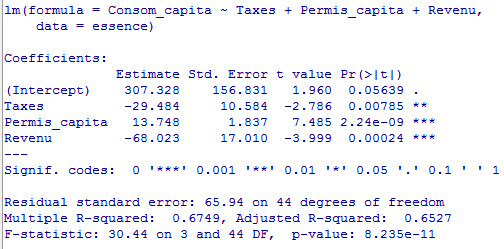
\includegraphics[width=10.5cm]{essence-rlm-3var.png}
\end{frame}


\begin{frame}[t]{Exemple sur la consommation d'essence}

{\small
On s'intéresse aux prédictions du modèle linéaire dans les conditions suivantes:

\begin{itemize}\itemsep0mm
\item taxe sur l'essence de 7 cents par gallon,
\item pourcentage de la population avec permis de conduire de 54\%
\item revenu per capita de 4000\$
%\item longueur des routes fédérales est 8 milliers de miles?
\end{itemize}
%

\begin{enumerate}[(i)]
\item Donnez un intervalle de confiance à 95\% pour la consommation d'essence par habitant \underline{en moyenne dans des états} où les conditions ci-dessus sont rencontrées.
\item Que devient votre prédiction et sa marge d'erreur si on remplace ``en moyenne dans des états'' dans la phrase précédente par ``\underline{dans un état en particulier}''?
\end{enumerate}
}
\end{frame}

\begin{frame}[t]{Exemple (suite)}

\begin{itemize}
\item[$\hat y_0$:] Estimation ponctuelle de $571,22$ gallons par habitant dans les deux cas
\item[i) ] intervalle pour la moyenne: $(542,69;\;599,76)$ gallons
\item[ii) ] intervalle pour une valeur individuelle: $(435,31;\;707,14)$ gallons
\end{itemize}

\medskip
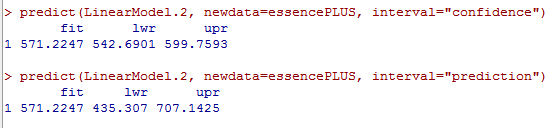
\includegraphics[width=8cm]{predict-3var.png}

\end{frame}
    


\section[Qualité]{Critères de qualité d'ajustement}

\subsection{Choix des variables à conserver}

\begin{frame}[t]{Sélection de variables }

{\small
\begin{itemize}\itemsep7mm
\item Trop de variables dans le modèle? \\{\it La variance des prévisions est trop grande. }
\item Manque de variables dans le modèle? \\{\it Les prévisions sont biaisées. }
\item Il existe  une multitude de \textit{critères servant à évaluer la qualité d'un modèle de régression}. \\ Deux critères se calculent à partir du tableau d'analyse de la variance: $R^2$ et $R^2_{ajuste}$.
\end{itemize}
}
\end{frame}

\begin{frame}[t]{Deux critères d'ajustement }

{\small
\begin{itemize}
\item<1-> \alert{Coefficient de détermination, $R^2$, proportion de la variation de $Y$ expliquée par le modèle}: $$R^2=\frac{SS_R}{SS_T}=1-\frac{SS_E}{SS_T}$$

    \underline{Problème pour la comparaison de modèles}: le $SS_R$ augmente toujours quand on ajoute des variables explicatives au modèle, même si elles sont inutiles...

\item<2-> \alert{Coefficient de détermination ajusté, $R^2_{ajuste}$}:
$$R^2_{ajuste}=1-\dfrac{SS_E/(n-k-1)}{SS_T/(n-1)}.$$

\underline{Plus approprié pour sélectionner les variables}.
\end{itemize}
}
\end{frame}

\begin{frame}[t]{Procédure de sélection de modèle}
Pour choisir les variables explicatives à retenir dans un modèle de régression:\\

\bigskip
\begin{enumerate}\itemsep5mm
\item ajuster tous les sous-modèles possibles et calculer $R^2_{ajuste}$ pour chacun d'entre eux;
\item conserver le modèle qui a le meilleur (\alert{plus grand}) $R^2_{ajuste}$.
\end{enumerate}
\end{frame}

\begin{frame}[t]{Exemple 4 sur la consommation d'essence}

D'après le $R^2_{ajuste}$, le meilleur sous-modèle est ...

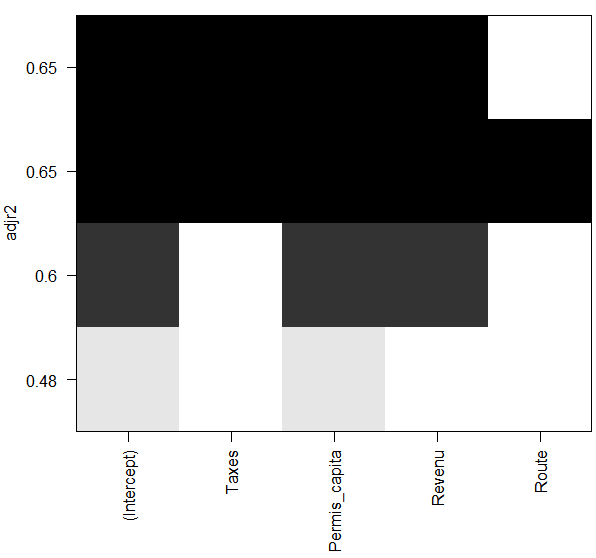
\includegraphics[width=6cm]{essence-choix.png}

\end{frame}


\begin{frame}[t]{ }


\centerline{\LARGE\bf \alert{QUIZ !}}
\bigskip

Vrai ou Faux ?



\begin{itemize}\itemsep1cm
\item La valeur du $MS_E$ est toujours plus petite pour un modèle contenant plus de variables.
\item La valeur du $MS_E$ diminue généralement quand on augmente la taille d'échantillon.
    \vspace{1cm}
\end{itemize}

\end{frame}

\begin{frame}[t]{Une autre approche}
    Le critère que nous venons de voir nous donne de l'information sur la \textit{qualité} du modèle. 
    
    Et si nous voulions plutôt avoir le meilleur modèle \alert{prédictif}?
\end{frame}


\begin{frame}[t]{Surajustement et généralisation}

{\small
Quand on utilise plusieurs variables explicatives, on risque de tomber dans le \alert{surajustement }.

\bigskip
\begin{itemize}\itemsep6mm
\item Le modèle prédit très bien les données qui ont servi à estimer celui-ci, mais \alert{échoue à bien prédire} de nouvelles données.
\item On aimerait plutôt construire un modèle qui prédit bien à de nouvelles observations.
\end{itemize}

\medskip
$\Rightarrow$ On a besoin d’\alert{outils pour estimer la performance prédictive réelle du modèle}.

\medskip

$\Rightarrow$ Nous n'avons qu'un seul jeu de données, que peut-on faire?
}
\end{frame}


\begin{frame}[t]{Validation croisée}

{\small
\alert{La validation croisée} est une méthode pour évaluer la performance prédictive d’un modèle à partir des données disponibles.

\bigskip

\begin{itemize}\itemsep5mm
\item On \alert{divise les données} en un ensemble d’entraînement et un ensemble de test (validation).
\item On \alert{ajuste le modèle sur l’ensemble d’entraînement}, puis on \alert{évalue l’erreur de prédiction} sur l’ensemble test.
\item Pour limiter l’effet du découpage, on répète cette opération plusieurs fois (ex: \alert{validation croisée en K plis}).
\end{itemize}

\bigskip
$\Rightarrow$ Fournit une estimation plus réaliste de la performance prédictive.
}
\end{frame}






\begin{frame}[t]{Implémentation de la validation croisée en K plis}

{\small
Pour calculer l'erreur de prédiction pour un modèle donné à l'aide de la validation croisée en K plis
\begin{itemize}
    \item[1.] Partitionner aléatoirement les $n$ observations du jeu de données en $K$ groupes.
    \item[2.] Pour \alert{chacun} des groupes 1 à $K$ :
    \begin{itemize}
        \item[(a)] Utiliser les données du groupe comme \alert{jeu de test} et les données
        des $K-1$ autres groupes comme \alert{jeu d'entrainement}.
        \item[(b)] Estimer les coefficients $\beta$ à partir du \alert{jeu d'entrainement}.
        \item[(c)] Utiliser les $\hat{\beta}$ obtenus en (b) et les $X$ des données
        du \alert{jeu de test} pour calculer les $\hat{Y}$ pour les données
        du \alert{jeu de test}.
        \item[(d)] Calculer $SSE_{\text{pred}}^{(k)}=\sum_{i\in\text{\alert{jeu de test}}}(\hat{Y}_i-Y_i)^2$.
    \end{itemize}
    \item[3.] Calculer $MSE_{\text{pred}}=\frac{1}{n}\sum_{k=1}^KSSE_{\text{pred}}^{(k)}$.
\end{itemize}
Les livres classiques de science des données (par exemple, \href{https://hastie.su.domains/ElemStatLearn/}{{\it Elements of Statistical Learning}}) recommandent souvent une valeur de $K=10$.
}
\end{frame}
\begin{frame}[t]{Exemple : sélection de variables avec validation croisée}

{\small
Supposons qu’on dispose de 4 variables explicatives \( X_1,\ldots,X_4 \). On veut déterminer lesquelles conserver dans le modèle pour maximiser la capacité de prédiction.

\bigskip

\begin{itemize}\itemsep3mm
\item On considère différents sous-modèles (ex: toutes les combinaisons possibles de variables).
\item Pour chaque modèle, on effectue une \alert{validation croisée en K plis} et on calcule l'erreur de prédiction moyenne (p.ex., MSE) [voir page suivante pour les détails].
\item On choisit le modèle avec la plus faible erreur de validation.
\end{itemize}
}

\end{frame}
\begin{frame}[t]{Exemple}

\begin{center}
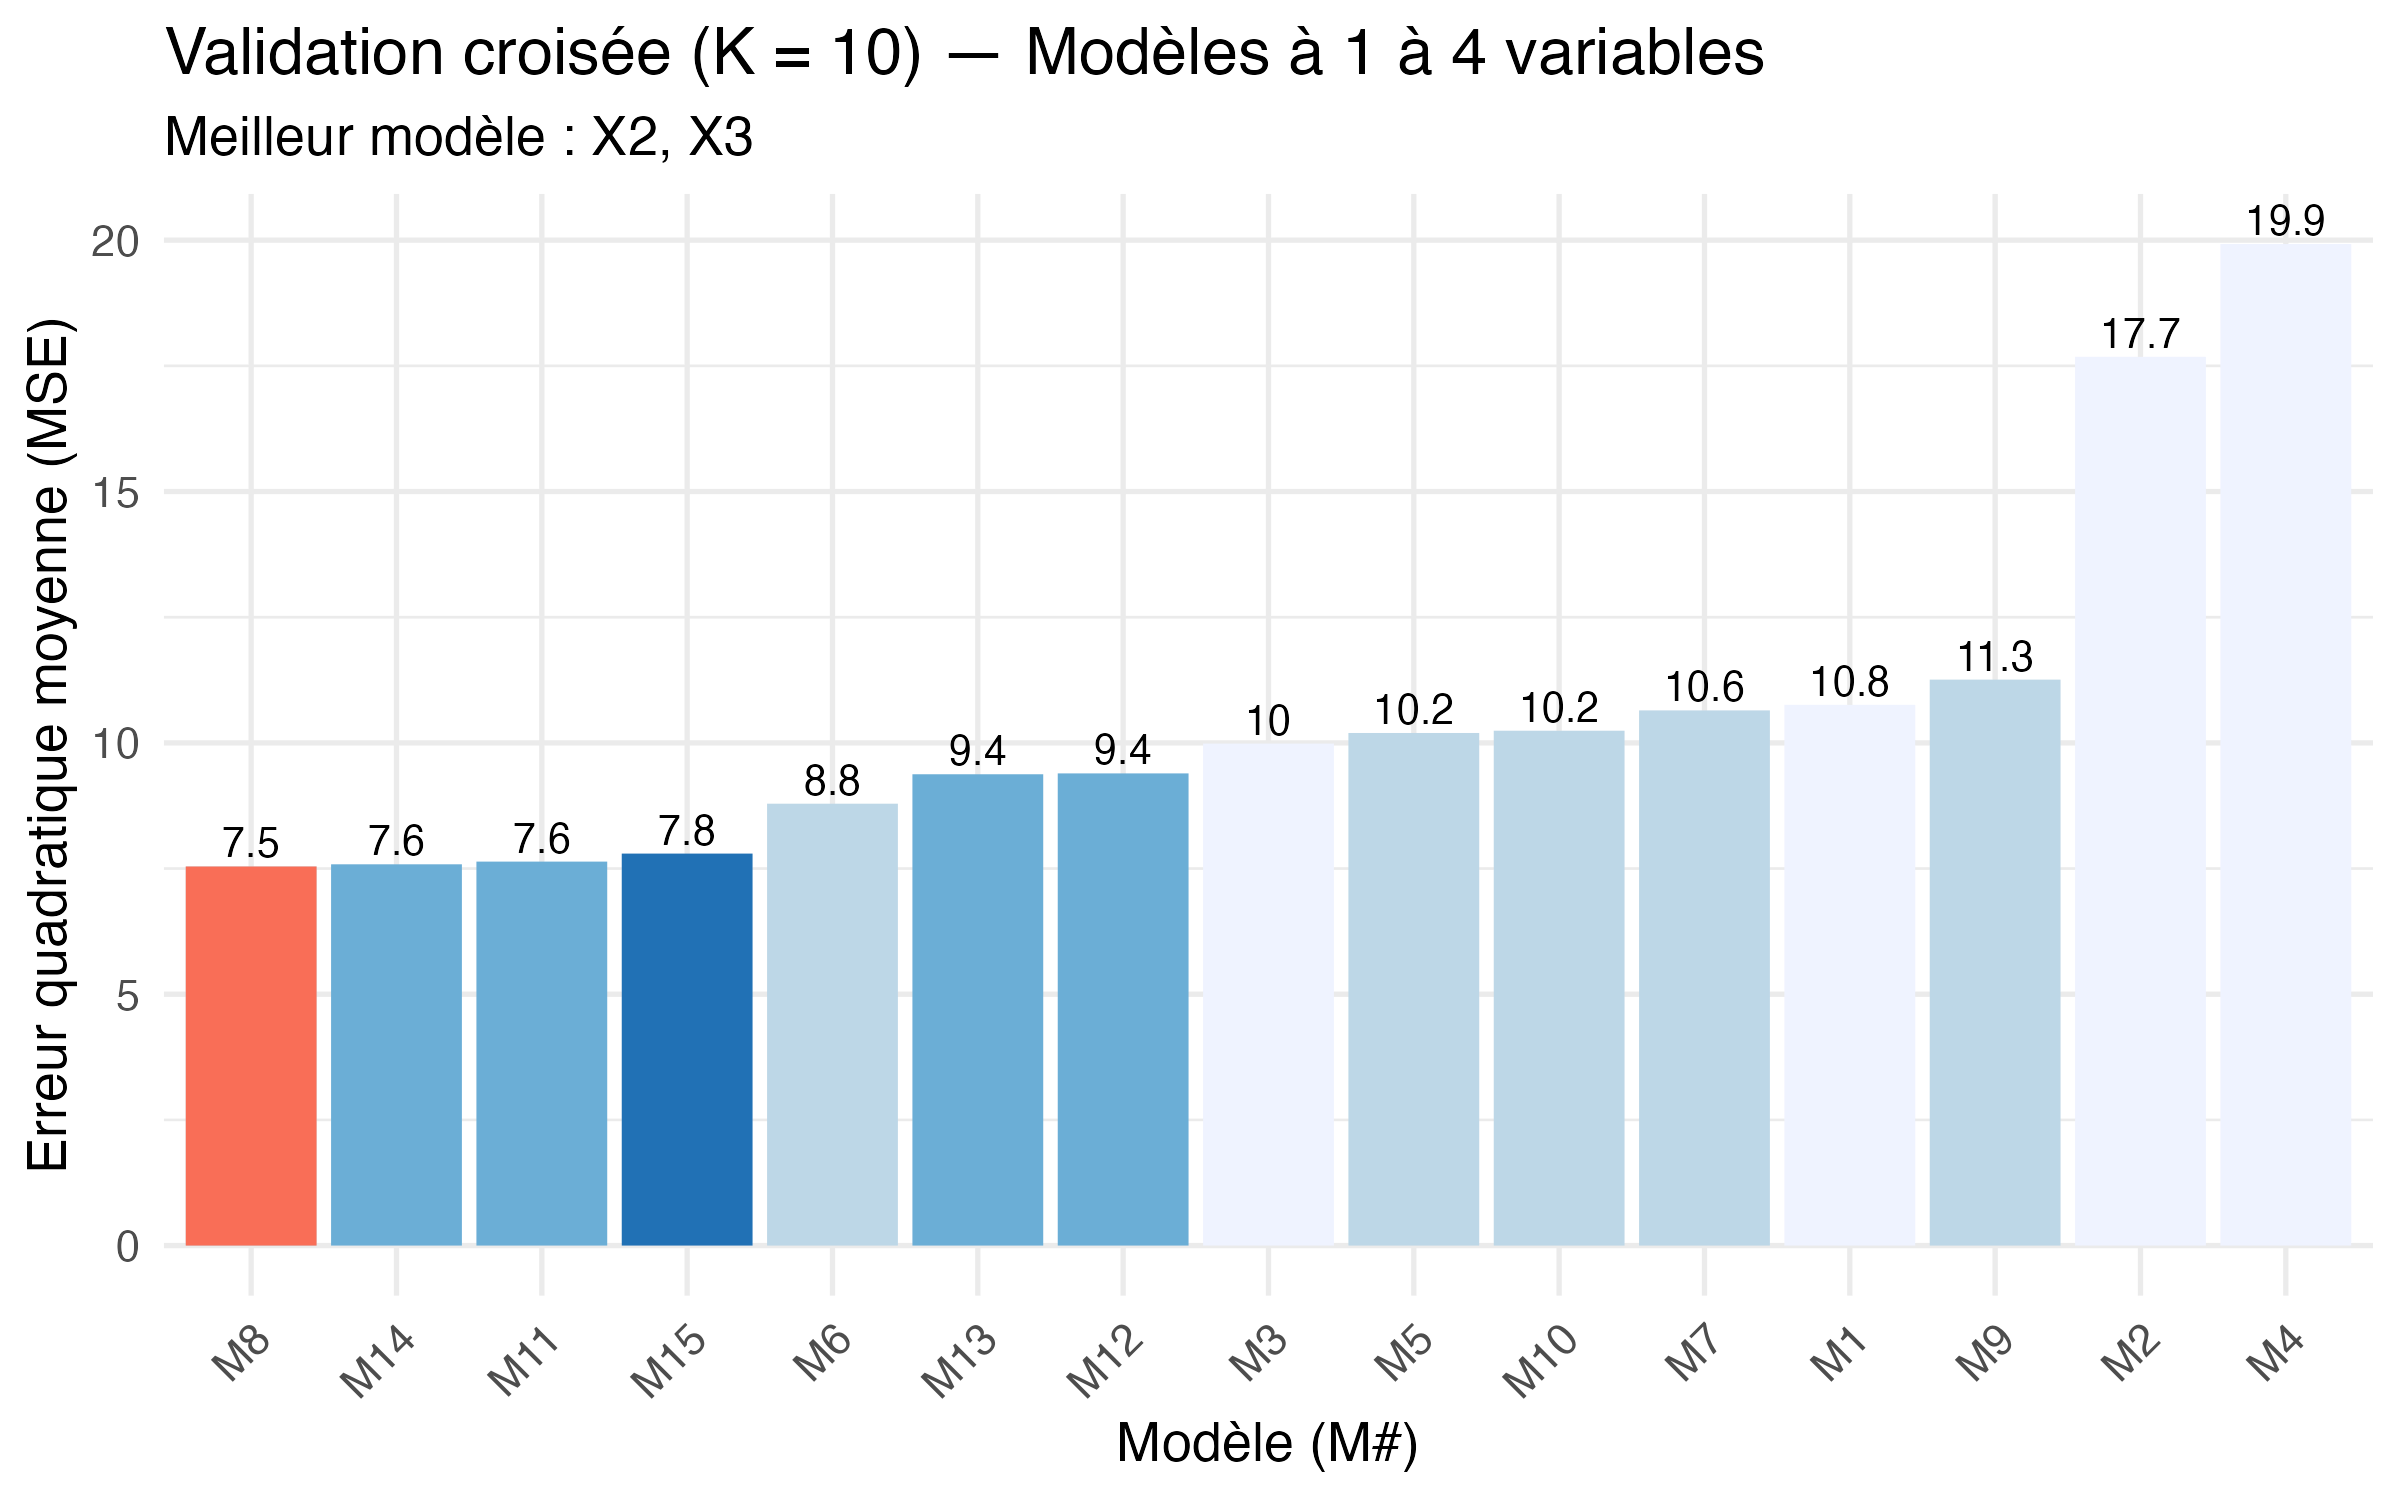
\includegraphics[width=0.85\textwidth]{Images/Module 11/valcroisee-selection.png}
\end{center}


\end{frame}


\begin{frame}[t]{Ouverture : vers l’apprentissage machine}

{\small
La régression linéaire multiple est un modèle simple mais fondamental.

\bigskip
Dans le contexte de grandes bases de données ou de relations complexes, d'autres méthodes sont souvent utilisées :

\begin{itemize}\itemsep4mm
\item arbres de décision, forêts aléatoires (random forests)
\item modèles à base de voisins (k-NN)
\item régularisation (ridge, lasso)
\item réseaux de neurones et autres méthodes d’apprentissage profond
\end{itemize}

\bigskip
\alert{Ces approches s’appuient toutes sur des techniques de validation croisée pour éviter le surajustement.}
}
\end{frame}
\section{Flexibilité du modèle}

\subsection*{}

\begin{frame}[t]{Flexibilité du modèle}

 \alert{\em Modèle linéaire}: lien linéaire  \alert{par rapport aux paramètres $\beta_0$ à $\beta_k$}. Sa formulation permet d'exprimer des relations très générales entre $Y$ et les $X_j$.

\medskip

\begin{itemize}\itemsep 7mm
\item relations polynomiales
\item modèle avec interaction entre les $X_j$
\item analyse de la variance
\item etc.
\end{itemize}

\end{frame}


\begin{frame}[t]{Exemple 6: Relation quadratique}

En posant $X_{1}=X$ et $X_{2}=X^2$, on a
\begin{align*}
Y&=\beta_0+\beta_1X_{1}+\beta_2X_{2}+E\\
&=\beta_0+\beta_1X+\beta_2X^2+E,
\end{align*}
soit une \alert{relation quadratique} entre $Y$ et $X$.


Quelle valeur de $X$ minimise la valeur moyenne de $Y$?

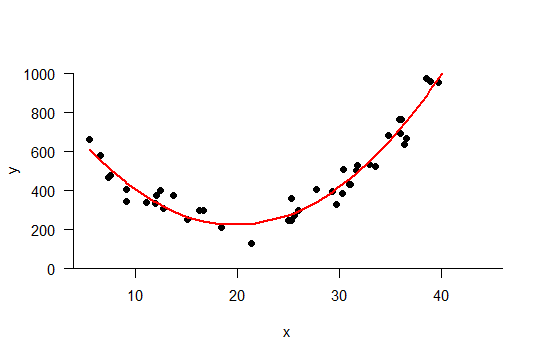
\includegraphics[width=6cm]{flex1.png}
\end{frame}

\begin{frame}[t]{Exemple 7: interactions entre deux variables explicatives}

On modélise l'interaction en posant $X_{3}=X_{1}X_{2}$ et
\begin{align*}
Y&=\beta_0+\beta_1X_{1}+\beta_2X_{2}+\beta_3X_{3}+E\\
&=\beta_0+\beta_1X_1+\beta_2X_{2}+\beta_3X_{1}X_{2}+E.
\end{align*}

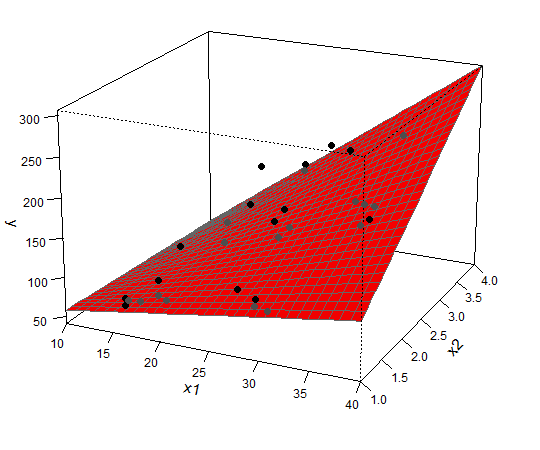
\includegraphics[width=6cm]{flex2.png}
\end{frame}

\begin{frame}[t]{Attention!}

{\small
\alert{En présence d'interaction ou de termes de degré supérieur, les coefficients ne s'interprètent pas de la même façon!}

Avec interaction,

$$Y=\beta_0+\beta_1X_1+\beta_2X_{2}+\beta_3X_{1}X_{2}+E,$$

si $X_2$ passe de 3 à 4 unités, l'effet sur $E[Y]$ est:
%\begin{align*}
%E[Y|X_2=x+1]-E[Y|X_2=x]&=\beta_0+\beta_1X_1+\beta_2(x+1)+\beta_3X_1(x+1)\\
%&\ \ \ -\left(\beta_0+\beta_1X_1+\beta_2x+\beta_3X_1x\right)\\
%&=\beta_2+\beta_3X_1,
%\end{align*}

\begin{align*}
E[Y|X_2=4]-E[Y|X_2=3]&=\beta_0+\beta_1X_1+\beta_2(4)+\beta_3X_1(4)\\
&\ \ \ -\left[\beta_0+\beta_1X_1+\beta_2(3)+\beta_3X_1(3)\right]\\
&=\beta_2+\beta_3X_1.
\end{align*}
Ainsi l'effet d'un changement dans la valeur de $X_2$ {\em dépend} de la valeur de $X_1$,
d'où le nom de ``terme d'interaction'' pour le terme $X_{1}X_{2}$.
}
\end{frame}

\begin{frame}[t]{Exemple 8: Lien avec l'analyse de la variance}

{\small
Supposons une expérience à un facteur à 3 niveaux (A, B et C). Posons

\medskip
$X_1=\left\{\begin{array}{ll}
1&\text{au niveau A}\\
0&\text{sinon}
\end{array}\right.
\quad \quad
X_2=\left\{\begin{array}{ll}
1&\text{au niveau B}\\
0&\text{sinon}
\end{array}\right.$

\medskip
Si on utilise le modèle linéaire avec  $E[Y|X_1,X_2]=\beta_0+\beta_1X_1+\beta_2X_2$, on retrouve le modèle d'analyse de la variance à un facteur.
}
\end{frame}


\begin{frame}[t]{Réponses aux exemples}

{\scriptsize

\begin{enumerate}\itemsep 1mm
  \item  Permis$\_$capita est la plus corrélée avec $Y=$ consommation d'essence. On ne peut pas déduire le meilleur modèle à plusieurs variables, car les coefficients dépendent de la présence des autres variables.
  \item $H_0$ rejetée. Au moins une des quatre variables explicatives est associée à la consommation d'essence.
  \item  Valeur-P pour Taxes $= 0,0103 < 0,05$. On rejette $H_0: \beta_1=0$, l'effet est significatif. \\
      Puisque  $10\;\in \; IC(\beta_2)$, on ne rejette pas  $H_0: \beta_2=10$.
  \item La ligne du haut représente le $R^2_{ajuste}$ maximal. On retient tout sauf Routes.
  \item $\hat Y_0=307.328-29.484(7)+13.748(54)-68.023(4) =571.22 $
  \item Le minimum de $E(Y)$ est atteint en  $x=-\beta_1/2\beta_2$.
  \end{enumerate}

 }
\end{frame}
\end{document}